\chapter{Introducci\'on}\label{cap:intro}

\begin{figure}[tbp]
\begin{center}
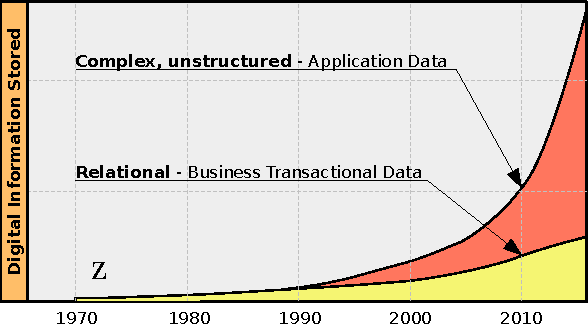
\includegraphics[width=0.99\textwidth]{imagenes/001.pdf}
 \caption{Demanda en crecimiento exponencial. Fuente: \emph{Cloudera Inc.}}
\label{fig:datagraph}
\end{center}
\end{figure}

\noindent Los \'ultimos a\~nos han visto c\'omo se ha producido una explosi\'on de la cantidad de informaci\'on generada en la red. Adem\'as, esta informaci\'on ha mudado de forma, pasando de \emph{semiestructurada} o \emph{estructurada} ---y por tanto, susceptible de ser expresada siguiendo un esquema tradicional (\emph{relacional}, por ejemplo)--- a heterog\'enea, lo que propicia la necesidad de cambiar el modo en que se almacena y eval\'ua. Como muestra la figura \ref{fig:datagraph}, las que hasta hace poco eran indiscutibles como \emph{backend} de datos, las bases de datos relacionales fundamentalmente, han visto c\'omo se difumina su papel principal ante la incapacidad de guardar eficazmente heterogeneidad no relacionada.\newline

En el a\~no 2000 fueron muchas las empresas del sector \emph{.com} que iniciaron remodelaciones de sus centros de datos para acomodarlos al entonces concebido como inexorable pico de demanda que iba a suceder. Pero se pincha la burbuja, desat\'andose una infrautilizaci\'on generalizada ---en Amazon s\'olo el \texttt{10\%} de los recursos globales estaban siendo utilizados--- que impulsa la b\'usqueda de alg\'un sistema que permita exportar el excedente como producto. La iniciativa de Amazon germina en 2006 con la aparici\'on de los \emph{AWS} (\emph{Amazon Web Services}), un API p\'ublico para el aprovisionamiento flexible y bajo demanda de infraestructura computacional.\newline

Desde entonces ha sido fant\'astica la proliferaci\'on de proyectos similares para generalizar el modo de utilizaci\'on de clusters privados, p\'ublicos o h\'ibridos, procurando mantener un notable paralelismo a nivel de API con los AWS, para facilitar la interoperabilidad y evitar la fuga hacia servicios m\'as flexibles de otros proveedores.\newline

Paralelamente, Google buscaba nuevas formas de explotar, con altas pres\-ta\-cio\-nes y de manera segura, la infraestructura privada adquirida para evolucionar su modelo de negocio. MapReduce, como mecanismo de ejecuci\'on masiva de procesos en paralelo, hac\'ia acto de presencia para impulsar la ge\-ne\-ra\-ci\'on del gigantesco \'indice inverso de Google \cite{googlemapreduce}. Aportaciones pos\-te\-rio\-res del equipo de desarrollo de Nutch ---entonces un prototipo de motor de b\'usqueda para Internet--- al paradigma MapReduce en \emph{Yahoo!}, dar\'ian lugar a la aparici\'on del hoy por hoy est\'andar de facto en el terreno: Hadoop. Hadoop se utiliza en la actualidad en multitud de \'ambitos como la con\-tra\-ta\-ci\'on de viajes online, el almacenamiento y servicio de datos a terminales m\'oviles, el comercio electr\'onico, el procesado de imagen o el descubrimiento de nuevas formas de energ\'ia.\newline

As\'i, sustentando la implementaci\'on de MapReduce sobre infraestructura \emph{el\'astica}, se conseguir\'ia la explotaci\'on \'optima de los recursos computacionales, expandi\'endolos o contray\'endolos r\'apidamente en funci\'on de la demanda, al tiempo que se reducir\'ia indirectamente el coste energ\'etico (ver figura \ref{fig:energysavings}) del servicio.

\begin{figure}[tbp]
\begin{center}
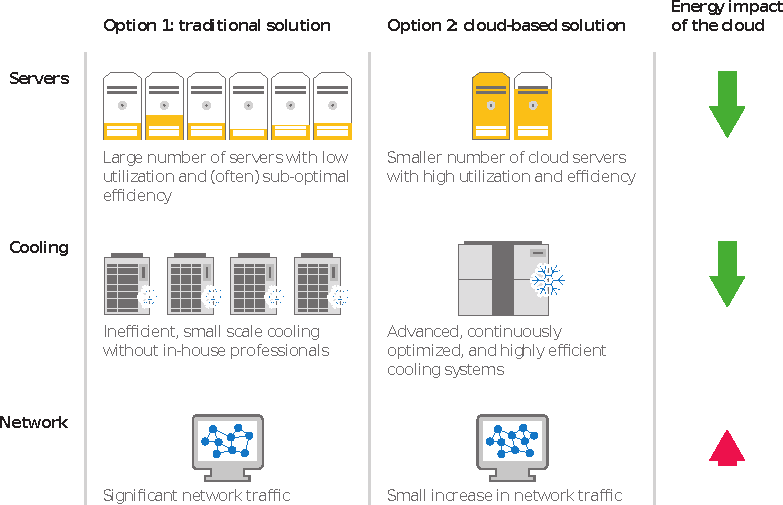
\includegraphics[width=0.99\textwidth]{imagenes/002.pdf}
 \caption{Motivaci\'on energ\'etica. Fuente: \cite{googleapps}}
\label{fig:energysavings}
\end{center}
\end{figure}



\section{Objetivos}\label{sec:objetivos}

\noindent El objetivo principal de este proyecto es estudiar la posibilidad de desarrollar una soluci\'on que permita dirigir el funcionamiento de un cloud para ejecutar algoritmia codificada siguiendo el paradigma MapReduce, reduciendo al m\'aximo la necesidad de conocimiento de la estructura del cloud concreto utilizado y de los par\'ametros de configuraci\'on de MapReduce.\newline

Para lograrlo se har\'a un an\'alisis pormenorizado de las variadas soluciones de creaci\'on de clouds. Se evaluar\'an sus capacidades y se configurar\'a un entorno de prueba utilizando virtualizaci\'on, que permita extraer conclusiones dirigidas a la elecci\'on de un \emph{framework} en concreto. Una vez completada la primera selecci\'on, se pasar\'a a la evaluaci\'on de los frameworks que soporten las caracter\'isticas del paradigma de programaci\'on MapReduce.\newline

Asimismo, se desarrollar\'a un mecanismo para el env\'io de peticiones de ejecuci\'on de trabajos MapReduce, centr\'andonos en la simplicidad y la universalidad de acceso de la interfaz con el cloud y MapReduce. Sin embargo, la sencillez no ha de representar un obst\'aculo para la explotaci\'on y la obtenci\'on de resultados. Del mismo modo, tanto la seguridad como la privacidad en las comunicaciones y el almacenamiento habr\'an de ser convenientemente definidas; no olvidemos que se trata la construcci\'on de un modelo reducido, a escala, de una soluci\'on que pueda ser implantable en una infraestructura infinitamente m\'as capaz.


\section{Organizaci\'on de la memoria}\label{sec:organizacion}
\noindent El contenido del presente documento se distribuye como se expone a continuaci\'on. Este primer cap\'itulo introduce la l\'inea general de desarrollo del proyecto. El cap\'itulo \ref{cap:estadodelarte} acerca al lector conceptos fundamentales de la \emph{computaci\'on cloud} ---como su arquitectura o la virtualizaci\'on--- y del paradigma MapReduce. El cap\'itulo \ref{cap:evaliaas} describe una evaluaci\'on pr\'actica de cuatro sistemas de manejo de clouds \emph{IaaS}. El cap\'itulo \ref{cap:openstack} explora la estructura modular y el funcionamiento particular de OpenStack Folsom. De forma an\'aloga, el cap\'itulo \ref{cap:hadoop} desvela las peculiarias de Hadoop como framework MapReduce. \newline

Los cap\'itulos subsiguientes se centran en detallar el proyecto desde distintos puntos de vista. El cap\'itulo \ref{cap:solucion} contiene las decisiones de dise\~no y los diagramas UML. El cap\'itulo \ref{cap:rendimiento} recoge los an\'alisis de rendimiento de la soluci\'on en un entorno real de pruebas. El cap\'itulo \ref{cap:conclusiones} analiza trabajos de investigaci\'on experimental relacionados con el proyecto, destacando comparativamente sus caracter\'isticas.  Finalmente, se resumen las principales aportaciones del proyecto y se proponen futuras mejoras a su implementaci\'on. \newline

Adicionalmente se han incluido dos anexos. El ap\'endice \ref{cap:guiainstalacion} recoge una gu\'ia r\'apida para la puesta en funcionamiento de una instalaci\'on del proyecto en un nodo. El ap\'endice \ref{cap:glosario} recoge las explicaciones de ciertos t\'erminos y tecnolog\'ias repartidas por todo el texto.
